\documentclass[fleqn]{article}

% If you're new to LaTeX, here's some short tutorials:
% https://www.overleaf.com/learn/latex/Learn_LaTeX_in_30_minutes
% https://en.wikibooks.org/wiki/LaTeX/Basics

% Formatting
\usepackage[utf8]{inputenc}
\usepackage[margin=1in]{geometry}


% Math
% https://www.overleaf.com/learn/latex/Mathematical_expressions
% https://en.wikibooks.org/wiki/LaTeX/Mathematics
\usepackage{amsmath,amsfonts,amssymb,mathtools}

% Images
% https://www.overleaf.com/learn/latex/Inserting_Images
% https://en.wikibooks.org/wiki/LaTeX/Floats,_Figures_and_Captions
\usepackage{graphicx,float}

% Tables
% https://www.overleaf.com/learn/latex/Tables
% https://en.wikibooks.org/wiki/LaTeX/Tables

% Algorithms
% https://www.overleaf.com/learn/latex/algorithms
% https://en.wikibooks.org/wiki/LaTeX/Algorithms
\usepackage[ruled,vlined]{algorithm2e}
\usepackage{algorithmic}

% Code syntax highlighting
% https://www.overleaf.com/learn/latex/Code_Highlighting_with_minted
\usepackage{minted}
\usemintedstyle{borland}



% References
% https://www.overleaf.com/learn/latex/Bibliography_management_in_LaTeX
% https://en.wikibooks.org/wiki/LaTeX/Bibliography_Management
\usepackage[backend=biber,style=apa, citestyle=apa]{biblatex}
\addbibresource{references.bib}
\usepackage[colorlinks,citecolor=blue,urlcolor=blue,bookmarks=false,hypertexnames=true]{hyperref} 


% To set vertical space between paragraphs
\setlength{\parskip}{1em}
% To set indents in paragraph
\setlength{\parindent}{0em}

% New command to cite with years in brackets
\newcommand{\mycite}[1]{\citeauthor{#1} (\citeyear{#1})}

% Title content
\title{A modeling approach to understand the dominant sediment phosphorus release mechanism in Jordan Lake}
\author{Smitom Swapna Borah}
\date{May 6, 2021}

\begin{document}

\maketitle


% Introduction and Overview
\section{Introduction}
Eutrophication has been a consistent global challenge to the management of different lakes, rivers and coastal locations. It can be broadly described as the excessive productivity in such water bodies on account of favorable natural or anthropogenic conditions leading to many detrimental ecological and socio-economic consequences \parencite{LeMoal2019}. Although different factors aid the eutrophication process, internal phosphorus release from the sediments has been regarded as one of its driving factors \parencite{Nurnberg2009}. Studies across the world have shown the significance of considering the internal phosphorus load for successful mitigation and restoration strategy of a lake or reservoir. One such success story is the restoration of Newman Lake, Washington where efforts were made not only for external phosphorus load reduction but also to control the internal phosphorus loading mechanism. Another successful restoration story is that of Tiefwarensee Lake, Germany which managed to control eutrophication by suppressing the internal phosphorus release. However, sediment phosphorus release is a complex subject and is far from being completely understood. The same strategies that appear effective for one lake may not be effective when applied to another lake. One such example is the restoration of Sempachersee Lake, Switzerland which despite adopting a strategy similar to Newman Lake failed to control the sediment phosphorus release \parencite{Nurnberg2009}.  

The complex nature of sediment phosphorus release can be attributed to the multitude of plausible release mechanisms that may or may not work simultaneously. Among these mechanisms, the iron oxyhydroxides-P binding mechanism is the most popular one \parencite{mortimer1942}. This simple model emphasizes the presence of oxic conditions over the sediment-water interface (SWI) for the maintenance of a thin FeOOH-P layer at the SWI. Under anoxic conditions, this layer might break down, leading to resuspension of sediment phosphorus into the water column. However, this mechanism may not be always dominant in a lake or reservoir. \mycite{Hupfer2008} have shown that sediment phosphorus release is also dependent on a variety of other factors such presence of substantial organic phosphorus in the sediment, presence of aluminum and calcium ions, microbial pool in the sediments and pH. These factors undermine the importance of oxygen in the hypolimnetic layer for phosphorus release from the sediments.

This study aims to understand the sediment phosphorus release mechanism that is dominant in Jordan Lake, North Carolina using three different sediment phosphorus release models: Zero-order model, First-order model and Hypoxic model. The Zero-order model is based on the assumption that phosphorus release from the sediments is a constant source of phosphorus loading, independent of hypoxic conditions in the overlying water and sediment phosphorus. The First-order model is based on the assumption that sediment phosphorus release is proportional to phosphorus content in the sediments. However, like the previous model, this model, too, ignores the hypoxic conditions for phosphorus resuspension. The Hypoxic model is another iteration of the Zero-order or First-order model, depending on the better performance of these models, which incorporates the hypoxic constraints in sediment phosphorus release. Evaluation of these models will provide a definitive insight into the driving phosphorus release mechanism in Jordan Lake. The best-performing model will be subsequently used to predict future phosphorus concentrations in the reservoir and investigate the role of sediment phosphorus release in such predictions.

\section{Methods}
\subsection{Study-area and data}
The models developed in this study are specific to Jordan Lake which is an artificial reservoir, located in Chatham County. It receives water from many tributaries such as Morgan Creek, New Hope Creek, Northeast Creek, White Oak Creek, Haw River, etc., and serves as a major source of water supply for the residents of the state. Based on the flow constriction points, the reservoir is divided into 4 segments to aid the modeling process. The Farrington Road causeway, Highway 64 causeway and narrows located southern part of the reservoir serve as the flow constriction points.

The data for this model has been taken from a variety of sources. The hydrologic data of the tributaries were obtained from USGS (2019)  and the water quality data for the lake and tributaries were obtained from the Water Quality Portal (2019). Additional data for this study were retrieved from the study carried out by \parencite{DelGuidice2019}. 

\subsection{Mathematical modeling}
To understand the phosphorus dynamics of Jordan Lake, each segment of the reservoir was assumed to be divided into 2 compartments: The water compartment and the sediment compartment (Figure. \ref{fig:conceptualmodel}).

% Conceptual diagram
\begin{figure}[ht]
    \centering
    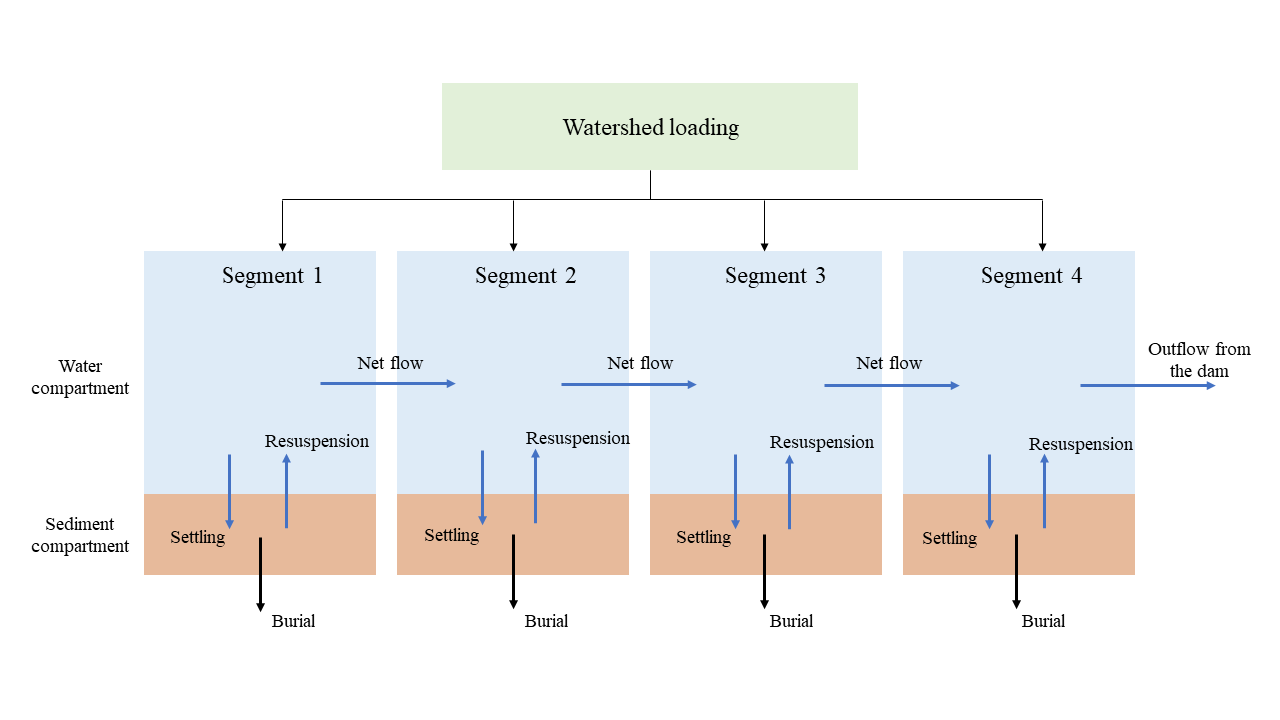
\includegraphics[width=0.9\linewidth]{Output/ConceptualDiagram.png}
    \caption{Conceptual diagram for the phosphorus model}
    \label{fig:conceptualmodel}
\end{figure}

The mass balance equation for phosphorus concentration in the lake in the water and sediment compartments can be written as follows:
\begin{equation}
    \frac{dM_i}{dt} = Resuspension + (Qin_i.Cin_i)(1-\psi)-M_i(k+\frac{v.A_i}{V_i})\theta_v^{T-20}+Q_{i-1,i}\frac{M_{i-1}}{V_{i-1}}-Q_{i,i+1}\frac{M_i}{V_i}
    \label{eqn:WaterMassbalance}
\end{equation}

\begin{flalign}
    \frac{dS_i}{dt} = S_i(k+\frac{v.A_i}{V_i})\theta_v^{T-20}-Resuspension-S_i.B_r
    \label{eqn:SedimentMassbalance}
\end{flalign}

The last two terms of the equation (\ref{eqn:WaterMassbalance}) can be replaced with terms, $Q_{i,i+1}\frac{M_{i+1}}{V_{i+1}}-Q_{i,i-1}\frac{M_i}{V_i}$ , in case the flow is reversed. The terms used in the above 2 equations are described as follows:\\
$M_i$ = Phosphorus mass in segment i of water compartment $[kg]$ \\
$S_i$ = Phosphorus mass in segment i of sediment compartment $[kg]$ \\
$v$ = Phosphorus transfer rate to the sediments (effective settling velocity) $[m/month]$\\
$k$ = Phosphorus transfer rate to the sediments (as a first-order removal rate) $[1/month]$\\
$\psi$ = Watershed nutrient load adjustment factor\\$B_r$ = Permanent burial rate from the sediments $[1/month]$\\
$\theta_v$ = Temperature adjustment factor for phosphorus transfer from water to sediments\\
$A_i$ = Surface water area of segment i $[10^6 m^2]$\\$V_i$ = Volume of water compartment of segment i $[10^6 m^3]$ \\
$Qin_i$ = Watershed inflow to segment i $[10^6 m^3/month]$ \\
$Cin_i$ = Phosphorus concentration in watershed inflow to segment i $[mg/m^3]$\\
$Q_{i-1,i}$ = Upstream flow to segment i $[10^6m^3/month]$ \\
$Q_{i,i+1}$ = Downstream flow from segment i $[10^6m^3/month]$

The resuspension term in equations (\ref{eqn:WaterMassbalance}) and (\ref{eqn:SedimentMassbalance}) was replaced by 3 sub-models which are described in the subsequent sections. The hydraulic flows between the segments and reservoir temperature were estimated by the methods described by \mycite{DelGuidice2019}. The differential equations were solved using the ‘odin’ package in R (FitzJohn, 2019)

\textbf{Zero-order sub-model}: In this sub-model, the sediment phosphorus was assumed to be released at a rate that is only dependent on temperature for a given segment. The resuspension sub-model can be written as:
\begin{equation}
    Resuspension = k_r.A_{si}.\theta_r^{(T-20)}
    \label{eqn:ZeroOrderModel}
\end{equation}
where $k_r$ is the phosphorus release flux from the sediments to the water compartment $[kg/m^2/month]$, $A_{si}$ is the sediment area $[m^2]$ of segment i and $\theta_r$ is the temperature adjustment factor. 

\textbf{First-order sub-model}: In this sub-model, the sediment phosphorus release flux was assumed to follow first-order rate kinetics: the resuspension of phosphorus from the sediments is dependent on the mass of sediment phosphorus at any given instant of time. Like the previous sub-model, the temperature-dependent nature of the resuspension was retained in this sub-model too. The first-order P release sub-model can be written as:
\begin{equation}
    Resuspension = R_s.S_i.\theta_r^{(T-20)}
    \label{eqn:FirstOrderModel}
\end{equation}
where $R_s$ is the recycling rate of sediment phosphorus $[1/month]$.\\
\textbf{Hypoxic sub-model}: The hypoxic sub-model is similar to the first-order P release sub-model which an exception that sediment phosphorus was assumed to be released only when hypoxic conditions appear to exist over the sediment-water interface (SWI). For this study, the hypoxia is assumed to prevail in the overlying water when dissolved oxygen level falls below 3 mg/L. It was also assumed that the recorded dissolved oxygen concentration at the maximum depth was an adequate representation of the dissolved oxygen conditions near the (SWI).  
\subsubsection{Model calibration}
The model parameters were calibrated in a Bayesian framework, using an adaptive Markov Chain Monte-Carlo approach. The ‘adaptMCMC’ package in R was used for this purpose (Scheidegger, 2018)

\newpage
% References
\printbibliography

\end{document}
